\chapter{User-controlled Shape Detection}
\newpage
\section{Overview}
The shape detection runs automatically in the background. It is designed in such a way that the user receives imminent feedback of local geometry for the region under the mouse cursor. The approach utilizes an automated shape detection algorithm that is capable of detecting different types of primitive shapes. This algorithm is designed to find shapes in point clouds that consist of several million points within minutes. However, when looking at the performance for smaller samples, results can be achieved at interactive time rates. Section \ref{sec:schnabel} describes the shape detection algorithm in detail. 
\\
Shape detection is performed one small regions only. Section \ref{sec:candidateNodes} describes a heuristic on how to choose such a region, using the user's cursor position and camera view as input. This effectively changes the task of shape detection from an automated approach to an user-controlled interaction.
\\ 
In order to use the detected shapes for rendering and interactions, the shapes must be postprocessed. Since some of the shapes are of infinite size, they need to be refitted to  encapsulate the corresponding support points and create a minimal boundary. Section\ref{sec:Refitting} describes this task. 

\section{Efficient RANSAC for Point-Cloud Shape Detection}
\label{sec:schnabel}
The section gives a brief overview over the algorithm used to detect primitive shapes. 
Schnabel et. al\cite{schnabel-2007-efficient} propose an automated way for detecting simple primitive shapes in unstructured point clouds. The point cloud is decomposed into a set of shapes and a set of unused points. The algorithm supports detection of planes, spheres, cylinders, cones, and tori. 

\textbf{RAN}dom \textbf{SA}mpling \textbf{C}onsens (RANSAC) was first discussed by Fischler and Bolles\cite{fischler1981random} as a paradigm for model fitting for image analysis and automated cartography. However, this approach can be generalized for points with an origin other than images. The shape detection utilizes RANSAC to repeatedly take a minimal set of points to build a primitive shape $\Psi$ and checks if the points in the region roughly follow the curvature of the shape. 

\subsection{Minimal sets}
A minimal set describes the set of points that is needed to construct a candidate shape. 
For each type of shape the following rule applies: A shape is only considered as candidate shape if all points from the minimal set are within a distance $\epsilon$ to the shape and the normal does not deviate from the shape's normal by more than an angle $\alpha$. 

\begin{itemize}
	\item \textbf{Plane}: A plane is constructed from three points $p_0, p_1, p_2$ whose normals do deviate from the plane's normal less than the angle $\alpha$. 
	
	\item \textbf{Sphere}: A sphere is fully defined by two points $p_0, p_1$ with corresponding normal vectors $n_0, n_1$. The center $c$ of the sphere is defined by the midpoint shortest line segment between the parametric lines $p_0 + tn_0$ and $p_1 + sn_1$. The radius is constructed by averaging the distance of $p_0$ and $p1$ to $c$.

	\item \textbf{Cylinder}:
	In order to create a cylinder a minimal set of two points  $p_0, p_1$ with corresponding normal vectors $n_0, n_1$ is used. The direction $d$ of the axis is established by $d = n_0 \times n_1$. The origin $c$ of the cylinder is created by projecting the parametric lines $p_0 + tn_0$ and $p_1 + sn_1$ onto the plane $d \cdot x = 0$ and taking their intersection as origin $c$. The radius is the shortest distance between $p_0$ and the axis $c + ud$
	
	\item \textbf{Cone}:
	For simplicity, the minimal set for a cone consists of three points $p_0, p_1, p_2$, rather than two. For each point-normal pair, a plane is created. The intersection of the three planes defines the apex $c$. To describe the direction of the axis a plane is constructed from the points \{$c +  \frac{p_0 - c}{||p_0 - c||}$, $c +  \frac{p_1 - c}{||p_1 - c||}$, $c +  \frac{p_2 - c}{||p_2 - c||}$\}. The normal of this plane is the direction $d$ of the cone axis. The opening angle is given as $\omega = \frac{\sum_{i}^{max} (p_i - c)\cdot d}{3}$
	
	\item \textbf{Torus}:
	A minimal set of four points with normals is used, one more than theoretically necessary However, this eases the computation.
	Two possible rotational axis are found by intersecting the four point-normal lines $p_i +  \lambda n_i$\cite{marshall2001robust}. For each axis a full torus is estimated and the torus is chosen that causes the smaller error in respect to the four points. The minor radius is found by projecting the points onto a plane that rotates around the axis. A circle is constructed using three points, whose radius is the minor radius of the torus. The major radius is given as the the distance of the circle center to the axis. 


\end{itemize} 

\subsection{Score function}
\label{sec:scorefun}
In order to only use points that roughly follow the curvature of a candidate shape, only points within a distance $\epsilon$ are taken into account Furthermore, each point must fulfill a score function in order to be considered a support point of the shape $\Psi$. 
The score function for each point consists of the following: 
\begin{itemize}
	\item The distance between the point and the shape must be smaller than $\epsilon$.
	\item The normal of the point must not deviate from the normal of the shape more than a given angle $\alpha$.
	\item Among all points that fulfill the previous two conditions, only the subset of points, that creates the largest connected component on the shape,  is considered.
\end{itemize}

All points that are within a distance $\epsilon$ are taken into account. However, only those whose normals do not deviate from the normal of the shape more than a given angle $\alpha$ are considered support points. Additionally, the number of support points must exceed a threshold value $n$ in order for this shape to be valid. 


\subsection{Performance}
\begin{table}
	\centering
	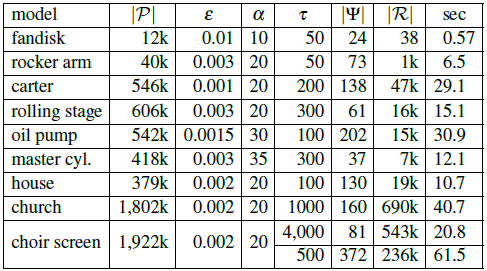
\includegraphics[width=0.7\textwidth]{Shape_Detection/schnabel-performance.png}
	\caption{The original statistics by Schnabel et. al\cite{schnabel-2007-efficient} on processed models. $\epsilon$ is given as ration of maximum bounding box with. Results have been averaged over 5 runs and rounded.}
	\label{table:schnabel_performance}
\end{table}

Table \ref{table:schnabel_performance} describes the statistical results for different models. $|P|$ is the number of points, $\epsilon$ the distance threshold, $\alpha$ the maximum normals deviation, $\tau$ is the minimum number of support points, $\|Psi|$ the number of shapes found, $|R|$ the number of RANSAC iterations. It can be seen that for small a small number of points and weaker constraints the algorithm returns plausible results within a fraction of a second. We utilize this feature the detect shapes in our application for small regions at a time to give immediate feedback to the user. 


\section{Selecting Candidate Nodes}
\label{sec:candidateNodes}
To select a proper candidate node from the octree, a node must fulfill the following constraints: 
\begin{itemize}
	\item The node must currently be rendered and visible to the user. 
	\item The node must contain at least $n$ points, the same amount used as minimal support point count for shape detection
	\item The node must not already contain detected shapes
\end{itemize}

Since this interaction is guided by the user, it makes sense that the user only interacts with what is presented on screen. Therefore the node must currently be rendered and visible. In order to eliminate overhead for the shape detection, the node must have enough points to at least fit one shape, otherwise it is ignored. Lastly, the shape detection algorithm works under the probabilistic assumption that all shapes were found, once it terminates. Therefore, nodes that already contain detected shapes are ignored as well. 
\\
The shape detection is guided by the user's cursor position. 
A raycast is performed, in order to select nodes that intersect with the cursor. 
The ray is constructed from the cursor's position on the near plane $p$ and the vector pointing from the camera to $p$. This ray is referred to as pick ray. 
An octree is an ideal data structure to perform a raycast. If the parent does not intersect the ray, neither will the children. This can be used to accelerate the process and prematurely eliminate nodes. The raycast on the octree can be performed with logarithmic cost. The raycast collects all nodes that intersect the pick ray. 

To choose the most suitable candidate node, all nodes from the raycast result are eliminated that do not fulfill the previous constraints. The LoD-level is larger the smaller the node is. The heuristic favors nodes with larger LoD-level so that the user receives geometric information for the most detailed parts of the currently explored region first. The projected distance to the nearplane is used to select between nodes with the same LoD-level. The node closest to the nearplane is favored. Algorithm ~\ref{alg:candidateNodeHeuristic} showcases the selection heuristic that is executed for each node that intersects the pick ray. It selects the node closest to the nearplane and the highest LoD-level.

\begin{algorithm}
	
	\KwData{raycastResults : OctreeNode[]}
	\KwResult{node : OctreeNode}
	node 	= null\;
	level = 0\;
	npd 	= 1.0\;
\ForEach{currentNode \normalfont{\textbf{in}} raycastResults}
	{
		isVisible = performViewFrustumCulling(node)\;
		\If{isVisible}{
			
			currentNpd = calculateDistanceToNearPlane(node)	\;
			currentLevel = node.getLodLevel()\;
			\If{currentLevel > level \normalfont{\textbf{or}} (currentLevel == level \normalfont{\textbf{and}} currentNpd < npd)}{
				node $\leftarrow$ currentNode\;
				level $\leftarrow$ currentLevel\;
				npd $\leftarrow$ currentNpd\;
				
			}
		}
	}
\caption{selectCandidateNode}
\label{alg:candidateNodeHeuristic}
\end{algorithm}

The selection of a suitable candidate node is highly dependent on the camera's position. When zooming out, the camera moves away from the scene, thus reducing the render horizon and therefore reducing the maximum level-of-detail. By ranking different nodes that fulfill the candidate criteria, even when the view does not change, a multi-scale representation of the local geometry is constructed over time, creating a level-of-detail for primitive shapes as well. 

\section{Refitting}
\label{sec:Refitting}
Planes, cylinder and cones are infinite shapes. Therefore, in order to use those shapes for rendering and interactions, it is necessary to create finite representations for each shape. Each shape comes with the corresponding set of support points that are used to refit the shape. Spheres and Tori are finite by definition. Therefore they do not require refitting. 

\subsection{Refitting planes}
Planes, however, are represented by a point and a vector. All support points are projected onto the plane, thus reducing the fitting problem to two dimensions. The procedure starts by computing the convex hull of the projected points with the help of Andrew's monotone chain 2d convex hull algorithm\cite{andrew1979another}. 
More complex polygons can be computed. However, for this purpose, a quad is sufficient. The quad is obtained by using the minimum-bounding-rectangle algorithm by Freeman\cite{freeman1975determining}. 

\subsection{Refitting cylinder}
A cylinder is defined by a center $p$, direction vector $v$ and a radius $r$. The height of the cylinder is infinite. To create a finite representation that encloses all support points, the two points whose difference in height is maximum. This is achieved by projecting all points onto the axis $a = p + vt$ of the cylinder, and select the points $p_{min}$, where $t$ is minimum and $p_{max}$, where $t$ is maximum. The distance $d$ between $p_{min}$ and $p_{max}$ is the height of the enclosing cylinder. The cylinder is refitted such that the new center is set to $p' = p_{min}$ and the $d$ is encoded in the length of the new direction vector:$v' = \frac{v}{|v|}d$. The radius stays the same. 

\subsection{Refitting cones}
A cone is defined by it's apex $c$, axis direction $v$ and opening angle $\theta$. Similar to the cylinder, all support points are projected to the axis and the points $p_{min}, p_{max}$ with minimum and maximum $t$ are selected. Since the apex of a cone is fixed, the range cannot be encoded using $c$ and $v$. The range is stored separately and range checks are performed when rendering or interacting with cones. 